\documentclass[../../../../main.tex]{subfiles}
\begin{document}

\begin{flushright}
\footnotesize\textit{【自動文字起こし・要確認】}
\end{flushright}

[解]

(1) 切り口は右図斜線部で、
これは一辺$\sqrt{2}t$の正三角形
だから
$$ T(t) = \frac{1}{2} \cdot \frac{\sqrt{3}}{2} (\sqrt{2}t)^2 = \frac{\sqrt{3}}{4} 2t^2 = \frac{\sqrt{3}}{2} t^2 \cdots (1) $$

\begin{center}
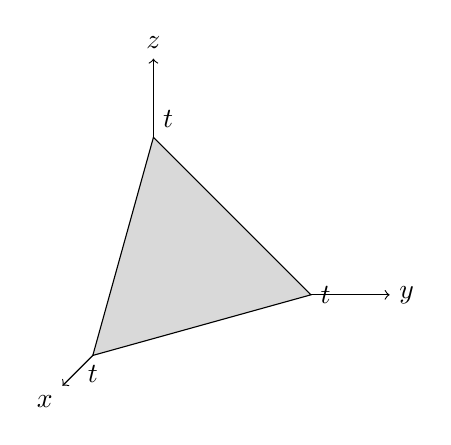
\begin{tikzpicture}[scale=1]
  \draw[->] (0,0,0) -- (3,0,0) node[right] {$y$};
  \draw[->] (0,0,0) -- (0,3,0) node[above] {$z$};
  \draw[->] (0,0,0) -- (0,0,3) node[below left] {$x$};
  \draw[fill=gray!30] (2,0,0) -- (0,2,0) -- (0,0,2) -- cycle;
  \node at (2,0,0) [right] {$t$};
  \node at (0,2,0) [above right] {$t$};
  \node at (0,0,2) [below] {$t$};
\end{tikzpicture}
\end{center}

(2)
(ア) $1 \le t \le 2$ の時
右図斜線部で、これは
一辺$\sqrt{2}t$の正三角形から
一辺$\sqrt{2}(t-1)$の " を
3つとりのぞいたもので、
$$ S(t) = \frac{\sqrt{3}}{2} t^2 - 3 \frac{\sqrt{3}}{2} (t-1)^2 = \frac{\sqrt{3}}{2} (-2t^2 + 6t - 3) $$

\begin{center}
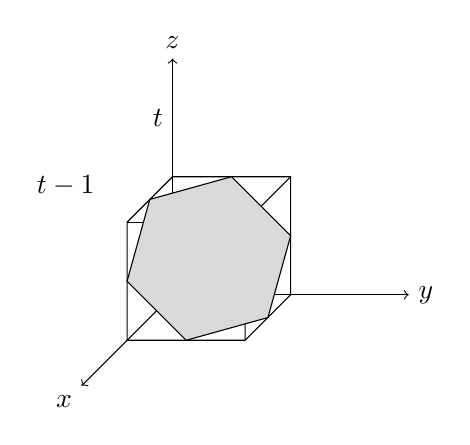
\begin{tikzpicture}[scale=1.5]
  \draw[->] (0,0,0) -- (2,0,0) node[right] {$y$};
  \draw[->] (0,0,0) -- (0,2,0) node[above] {$z$};
  \draw[->] (0,0,0) -- (0,0,2) node[below left] {$x$};
  \draw (1,0,1) -- (1,0,0) -- (1,1,0) -- (0,1,0) -- (0,1,1) -- (0,0,1) -- cycle;
  \draw (1,0,1) -- (1,1,1) -- (1,1,0);
  \draw (0,1,1) -- (1,1,1);
  \coordinate (A) at (1, 0, 0.5);
  \coordinate (B) at (1, 0.5, 0);
  \coordinate (C) at (0.5, 1, 0);
  \coordinate (D) at (0, 1, 0.5);
  \coordinate (E) at (0, 0.5, 1);
  \coordinate (F) at (0.5, 0, 1);
  \draw[fill=gray!30] (A) -- (B) -- (C) -- (D) -- (E) -- (F) -- cycle;
  \node at (0, 1.5, 0) [left] {$t$};
  \node at (0, 1.5, 1.5) [left] {$t-1$};
\end{tikzpicture}
\end{center}

(イ) $2 \le t < 3$ の時
右図斜線部で、これは
一辺$\sqrt{2}(3-t)$の正三角形で、
$$ S(t) = \frac{\sqrt{3}}{2} (3-t)^2 $$

\begin{center}
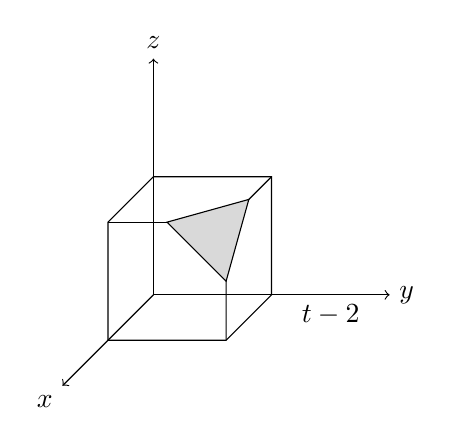
\begin{tikzpicture}[scale=1.5]
  \draw[->] (0,0,0) -- (2,0,0) node[right] {$y$};
  \draw[->] (0,0,0) -- (0,2,0) node[above] {$z$};
  \draw[->] (0,0,0) -- (0,0,2) node[below left] {$x$};
  \draw (1,0,1) -- (1,0,0) -- (1,1,0) -- (0,1,0) -- (0,1,1) -- (0,0,1) -- cycle;
  \draw (1,0,1) -- (1,1,1) -- (1,1,0);
  \draw (0,1,1) -- (1,1,1);
  \coordinate (A) at (1, 0.5, 1);
  \coordinate (B) at (1, 1, 0.5);
  \coordinate (C) at (0.5, 1, 1);
  \draw[fill=gray!30] (A) -- (B) -- (C) -- cycle;
  \node at (1.5, 0, 0) [below] {$t-2$};
\end{tikzpicture}
\end{center}

(ウ) $0 < t \le 1$ の時
明らかに $S(t) = T(t) = \frac{\sqrt{3}}{2} t^2$

以上から、$y=S(t)$のグラフは下図

\begin{center}
\begin{tikzpicture}
  \draw[->] (-0.5, 0) -- (4, 0) node[right] {$t$};
  \draw[->] (0, -0.5) -- (0, 3) node[above] {$y$};
  \draw[domain=0:1, smooth, variable=\x] plot ({\x}, {0.866*\x*\x});
  \draw[domain=1:2, smooth, variable=\x] plot ({\x}, {0.866*(-2*\x*\x + 6*\x - 3)});
  \draw[domain=2:3, smooth, variable=\x] plot ({\x}, {0.866*(3-\x)*(3-\x)});
  \draw[dashed] (1, 0) node[below] {$1$} -- (1, 0.866) -- (0, 0.866) node[left] {$\frac{\sqrt{3}}{2}$};
  \draw[dashed] (1.5, 0) node[below] {$\frac{3}{2}$} -- (1.5, 1.299) -- (0, 1.299) node[left] {$\frac{3\sqrt{3}}{4}$};
  \draw[dashed] (2, 0) node[below] {$2$} -- (2, 0.866);
  \node at (3, 0) [below] {$3$};
  \node at (0, 0) [below left] {$O$};
\end{tikzpicture}
\end{center}

よって、$\max S(t) = S\left(\frac{3}{2}\right) = \frac{3\sqrt{3}}{4}$

\end{document}
